\documentclass[letterpaper]{article}
\usepackage[submission]{aaai2027}
\usepackage[hyphens]{url}
\usepackage{graphicx}
\urlstyle{rm}
\def\UrlFont{\rm}
\usepackage{natbib}
\usepackage{caption}
\frenchspacing
\usepackage{booktabs}
\usepackage{multirow}
\usepackage{amsmath,amssymb}

\pdfinfo{
/TemplateVersion (2027.1)
}

\setcounter{secnumdepth}{0}

\title{Supplementary Material for PACT: Identity-Preserving Domain-Incremental Adaptation of Frozen Time-Series Foundation Models}
\author{Anonymous Submission}
\affiliations{}

\begin{document}

\maketitle

\section{Proof of Proposition 1}

\emph{Proof.}
Let $u=\hat z-z$. By the inference rule, the triangle inequality, the clipping
condition $\lVert\Delta^{d}_{c}(z)\rVert_2\le B$, and
$\sum_{d=1}^{T}\pi_{c,d}(z)=1-\pi_{c,0}(z)$,
\begin{align}
\lVert u\rVert_2
&\le
\sum_{c=1}^{K} w_c(z)
\sum_{d=1}^{T}\pi_{c,d}(z)\,
\big\lVert \Delta^{d}_{c}(z)\big\rVert_2 \notag\\
&\le
B \sum_{c=1}^{K} w_c(z)\big(1-\pi_{c,0}(z)\big)
= B\big(1-\pi_0(z)\big).
\end{align}
Since every logit is $L$-Lipschitz, each logit changes by at most
$L\lVert u\rVert_2$. The true-class margin after routing is therefore at least
$m(z)-2L\lVert u\rVert_2$. If
$(1-\pi_0(z))B<m(z)/(2L)$, the post-routing margin remains positive and the
predicted class is unchanged. If $\pi_0(z)=1$, then all non-source
responsibility vanishes on charts with nonzero membership, so $u=0$ and the
prediction is exactly the frozen-host prediction. \hfill$\square$

\section{Supplementary Figures}

\begin{figure*}[t]
\centering
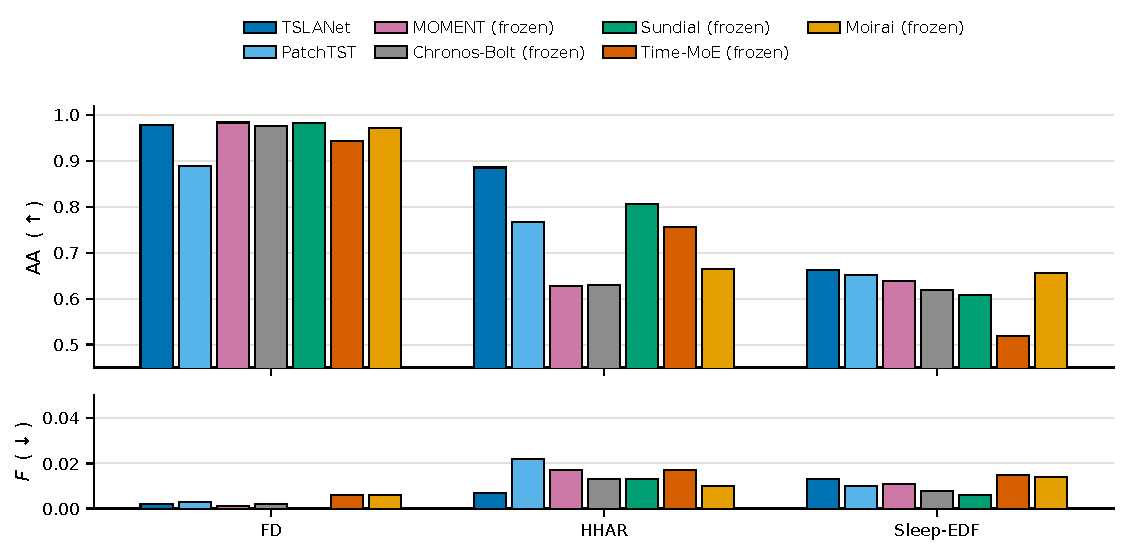
\includegraphics[width=\textwidth]{figures/fig_backbones.pdf}
\caption{\textbf{PACT across seven backbones on the domain-incremental chain.}
Top: average macro-$F_1$ (AA). Bottom: forgetting $F$, which remains low across
specialist encoders and frozen TSFMs.}
\label{fig:backbones}
\end{figure*}

\begin{figure*}[t]
\centering
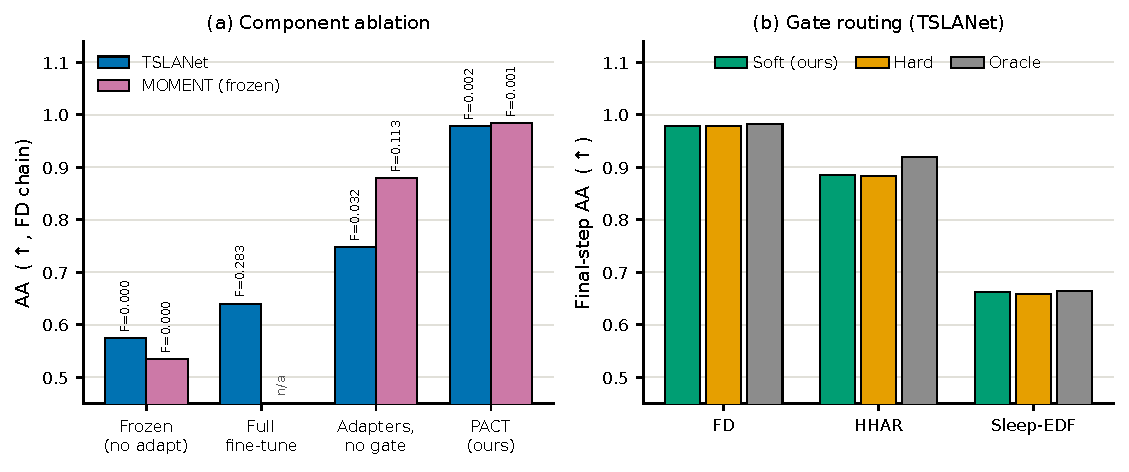
\includegraphics[width=\textwidth]{figures/fig_ablation.pdf}
\caption{\textbf{Ablations.} (a) Component ablation on the FD chain:
macro-$F_1$ climbs across variants, but only PACT keeps forgetting near zero.
(b) Gate routing: soft mixture tracks the oracle ceiling; the residual
soft--oracle gap is largest on HHAR.}
\label{fig:ablation}
\end{figure*}

\begin{figure*}[t]
\centering
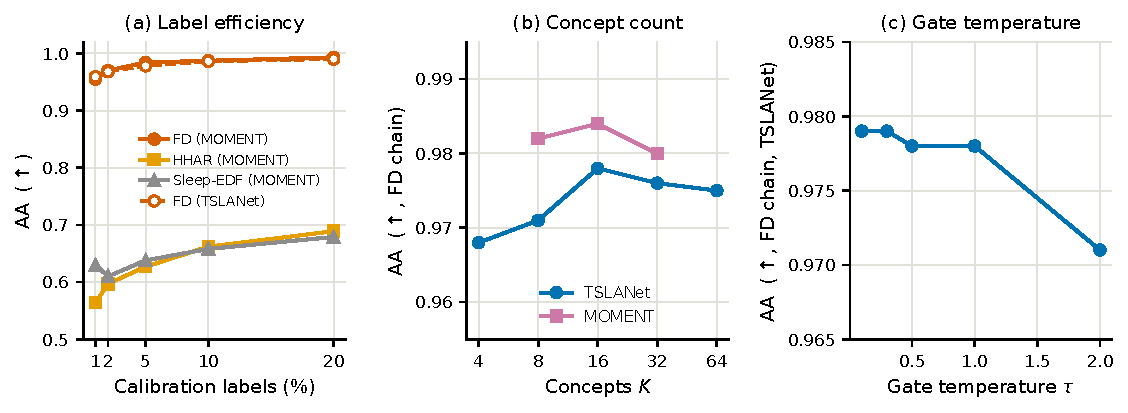
\includegraphics[width=\textwidth]{figures/fig_robustness.pdf}
\caption{\textbf{Robustness and label efficiency.} Average macro-$F_1$ is
stable across calibration budget, chart count, and gate temperature; forgetting
stays near zero throughout the sweeps.}
\label{fig:robustness}
\end{figure*}

% =====================================================================
% SUPPLEMENT -- FULL RESULT TABLES
% Included by supplement.tex.
% Requires: booktabs, multirow (same as paper_tables.tex).
%
% This is paper_tables.tex (Tables 1-7, verbatim) relocated under one
% supplement section, with Table 6 replaced: the original packed
% slash-separated version rendered with stretched column gaps, so it is
% swapped here for an expanded one-row-per-setting layout. That also let
% us report the real per-row F instead of only a "<= x" ceiling, and in
% doing so we caught a rounding slip in the source summary: the TSLANet
% 2% label-budget AA is 0.967 (from sweep_budget_tslanet.csv), not 0.968
% as listed in ALL_TABLES.md / the old Table 6 -- fixed below. Every
% other cell was re-checked against the raw sweep_*.csv files and matches.
% =====================================================================

\section{Full Result Tables}
\label{app:full-tables}
This supplement reports the complete per-method numbers underlying the
figures in the main paper. Table~\ref{tab:main-pairwise} is the
pairwise AdaTime benchmark; Tables~\ref{tab:chain-tslanet}--\ref{tab:budget-moment}
are the domain-incremental chain. Recall the two protocols differ: pairwise
adapts a single source$\rightarrow$target shift, whereas the chain
accumulates domains sequentially, so numbers are not directly comparable
across the two (e.g.\ source-distillation on FD is $0.923$ pairwise vs.\
$0.573$ on the 4-domain chain).

% ---------------------------------------------------------------------
% TABLE 1 — MAIN COMPARISON vs BASELINES (pairwise AdaTime, TSLANet)
% ---------------------------------------------------------------------
\begin{table*}[t]
\centering
\caption{Comparison on the AdaTime cross-domain benchmark (TSLANet backbone,
averaged over 10 source$\rightarrow$target shifts per dataset).
AA$\uparrow$ is average macro-$F_1$; BWT is the mean final-minus-first-seen
change on prior domains; $F$ is its nonnegative drop counterpart
($\downarrow$, 0 = no forgetting). Best AA per dataset in \textbf{bold}.
\textsuperscript{\dag}semi-supervised UDA using the same 5\% labeled target
split as PACT.}
\label{tab:main-pairwise}
\small
\begin{tabular}{l ccc ccc ccc}
\toprule
& \multicolumn{3}{c}{FD} & \multicolumn{3}{c}{HHAR} & \multicolumn{3}{c}{Sleep-EDF}\\
\cmidrule(lr){2-4}\cmidrule(lr){5-7}\cmidrule(lr){8-10}
Method & AA & BWT & $F$ & AA & BWT & $F$ & AA & BWT & $F$\\
\midrule
\multicolumn{10}{l}{\textit{No adaptation}}\\
Source-only & 0.839 & 0.000 & 0.000 & 0.742 & 0.000 & 0.000 & 0.670 & 0.000 & 0.000\\
\midrule
\multicolumn{10}{l}{\textit{Unsupervised domain adaptation}}\\
DANN & 0.865 & $-$0.027 & 0.027 & 0.762 & $-$0.012 & 0.012 & 0.676 & $-$0.019 & 0.021\\
Deep CORAL & 0.831 & $-$0.014 & 0.014 & 0.784 & $-$0.004 & 0.004 & 0.673 & $+$0.001 & 0.007\\
MMDA & 0.834 & $-$0.016 & 0.016 & 0.741 & $-$0.007 & 0.007 & 0.615 & $-$0.007 & 0.016\\
TENT & 0.840 & $-$0.008 & 0.008 & 0.727 & $-$0.006 & 0.006 & 0.663 & $-$0.007 & 0.009\\
DANN\textsuperscript{\dag} & 0.886 & $-$0.060 & 0.060 & 0.951 & $-$0.010 & 0.010 & 0.706 & $-$0.015 & 0.018\\
CDAN\textsuperscript{\dag} & 0.848 & $-$0.072 & 0.072 & \textbf{0.953} & $-$0.012 & 0.012 & 0.671 & $-$0.049 & 0.049\\
\midrule
\multicolumn{10}{l}{\textit{Fine-tuning references}}\\
Full fine-tune & 0.810 & $-$0.291 & 0.291 & 0.806 & $-$0.337 & 0.337 & 0.650 & $-$0.179 & 0.179\\
Head fine-tune & 0.846 & $-$0.010 & 0.010 & 0.801 & $-$0.067 & 0.067 & 0.657 & $-$0.124 & 0.124\\
\midrule
\multicolumn{10}{l}{\textit{Continual learning}}\\
EWC & 0.817 & $-$0.263 & 0.263 & 0.812 & $-$0.183 & 0.183 & 0.677 & $-$0.001 & 0.003\\
LwF & 0.806 & $-$0.220 & 0.220 & 0.852 & $-$0.113 & 0.113 & 0.666 & $-$0.105 & 0.105\\
MAS & 0.839 & 0.000 & 0.000 & 0.743 & 0.000 & 0.000 & 0.673 & 0.000 & 0.002\\
Source-distill & 0.923 & $-$0.004 & 0.004 & 0.961 & $-$0.001 & 0.001 & \textbf{0.721} & $-$0.020 & 0.020\\
\midrule
\multicolumn{10}{l}{\textit{Ours}}\\
PACT (no gate) & 0.933 & $-$0.106 & 0.106 & 0.854 & $-$0.210 & 0.210 & 0.648 & $-$0.162 & 0.162\\
\textbf{PACT (ours)} & \textbf{0.981} & 0.000 & 0.000 & \textbf{0.963} & $-$0.001 & 0.001 & 0.715 & $-$0.004 & 0.005\\
\bottomrule
\end{tabular}
\end{table*}

% ---------------------------------------------------------------------
% TABLE 2A — CHAIN CONTINUAL BASELINES (TSLANet)
% ---------------------------------------------------------------------
\begin{table*}[t]
\centering
\caption{Domain-incremental chain comparison, Part~A: TSLANet backbone.
Domains arrive sequentially (AdaTime-derived order; FD 4, HHAR 9, Sleep 17).
All methods use the same 5\% labelled calibration budget per domain as PACT
(ORTCL (LF) uses rotation only; ORTCL+HeadFT uses 5\% calib for head fine-tuning).
AA$\uparrow$; $F$$\downarrow$. Best AA per dataset in \textbf{bold}.
\textsuperscript{$\ddagger$}ORTCL: SVD rotation on last TSLANet ICB layer at each domain step.
Underlies the main trade-off figure.}
\label{tab:chain-tslanet}
\small
\begin{tabular}{l ccc ccc ccc}
\toprule
& \multicolumn{3}{c}{FD} & \multicolumn{3}{c}{HHAR} & \multicolumn{3}{c}{Sleep-EDF}\\
\cmidrule(lr){2-4}\cmidrule(lr){5-7}\cmidrule(lr){8-10}
Method & AA & $F$ & RF & AA & $F$ & RF & AA & $F$ & RF\\
\midrule
Frozen (no adapt) & 0.574 & 0.000 & 0.000 & 0.349 & 0.000 & 0.000 & 0.622 & 0.000 & 0.000\\
Full fine-tune & 0.640 & 0.283 & 0.295 & 0.654 & 0.345 & 0.360 & 0.584 & 0.116 & 0.178\\
Head fine-tune & 0.586 & 0.012 & 0.028 & 0.576 & 0.133 & 0.194 & 0.605 & 0.056 & 0.105\\
EWC & 0.590 & 0.001 & 0.003 & 0.526 & 0.093 & 0.177 & 0.620 & 0.004 & 0.012\\
MAS & 0.601 & 0.057 & 0.057 & 0.653 & 0.280 & 0.311 & 0.605 & 0.052 & 0.101\\
LwF & 0.549 & 0.256 & 0.257 & 0.723 & 0.155 & 0.194 & 0.622 & 0.026 & 0.067\\
Source-distill & 0.573 & 0.256 & 0.256 & 0.482 & 0.083 & 0.149 & 0.622 & 0.026 & 0.055\\
ORTCL (LF)\textsuperscript{$\ddagger$} & 0.538 & 0.004 & 0.006 & 0.375 & 0.009 & 0.109 & 0.370 & 0.091 & 0.307\\
ORTCL+HeadFT\textsuperscript{$\ddagger$} & 0.582 & 0.011 & 0.020 & 0.563 & 0.139 & 0.182 & 0.458 & 0.093 & 0.234\\
\textbf{PACT (ours)} & \textbf{0.978} & 0.002 & 0.002 & \textbf{0.886} & 0.007 & 0.011 & \textbf{0.663} & 0.013 & 0.033\\
\bottomrule
\end{tabular}
\end{table*}

% ---------------------------------------------------------------------
% TABLE 2B — CHAIN CONTINUAL BASELINES (frozen MOMENT)
% ---------------------------------------------------------------------
\begin{table*}[t]
\centering
\caption{Domain-incremental chain comparison, Part~B: frozen TSFM backbone
(AutonLab/MOMENT-1-large). Encoder frozen; only the linear head is updated
(head-FT / EWC / MAS / LwF / source-distill). Full-host methods are omitted
because the target setting requires the TSFM host to remain frozen. Same 5\%
calibration budget. AA$\uparrow$; $F$$\downarrow$. On HHAR, LwF (head)
reaches marginally higher AA than PACT (0.646 vs.\ 0.627) but at roughly
$3\times$ the forgetting ($F$: 0.050 vs.\ 0.017), the one case where a
baseline is not strictly dominated.}
\label{tab:chain-moment}
\small
\begin{tabular}{l ccc ccc ccc}
\toprule
& \multicolumn{3}{c}{FD} & \multicolumn{3}{c}{HHAR} & \multicolumn{3}{c}{Sleep-EDF}\\
\cmidrule(lr){2-4}\cmidrule(lr){5-7}\cmidrule(lr){8-10}
Method & AA & $F$ & RF & AA & $F$ & RF & AA & $F$ & RF\\
\midrule
Frozen (no adapt) & 0.535 & 0.000 & 0.000 & 0.525 & 0.000 & 0.000 & 0.635 & 0.000 & 0.000\\
Head fine-tune & 0.856 & 0.139 & 0.143 & 0.600 & 0.152 & 0.202 & 0.552 & 0.159 & 0.228\\
EWC (head) & 0.632 & 0.006 & 0.014 & --- & --- & --- & --- & --- & ---\\
MAS (head) & 0.874 & 0.065 & 0.072 & --- & --- & --- & --- & --- & ---\\
LwF (head) & 0.859 & 0.033 & 0.034 & 0.646 & 0.050 & 0.071 & 0.619 & 0.052 & 0.086\\
Source-distill (head) & 0.749 & 0.028 & 0.030 & 0.597 & 0.070 & 0.108 & 0.626 & 0.048 & 0.081\\
Adapters, no gate & 0.879 & 0.113 & 0.116 & 0.632 & 0.035 & 0.051 & 0.606 & 0.016 & 0.032\\
\textbf{PACT (ours)} & \textbf{0.984} & 0.001 & 0.001 & 0.627 & \textbf{0.017} & \textbf{0.027} & \textbf{0.638} & \textbf{0.011} & \textbf{0.031}\\
\bottomrule
\end{tabular}
\end{table*}

% ---------------------------------------------------------------------
% TABLE 3 — PACT IS BACKBONE-AGNOSTIC (chain, all backbones)
% ---------------------------------------------------------------------
\begin{table*}[t]
\centering
\caption{PACT across backbones on the domain-incremental chain (base config:
$K{=}16$, 5\% calibration, identity adapters). Specialist classifiers and
frozen TSFMs both achieve near-zero forgetting. AA$\uparrow$; $F$/RF$\downarrow$.
Underlies the supplementary backbone figure.}
\label{tab:backbones}
\small
\begin{tabular}{l ccc ccc ccc}
\toprule
& \multicolumn{3}{c}{FD} & \multicolumn{3}{c}{HHAR} & \multicolumn{3}{c}{Sleep-EDF}\\
\cmidrule(lr){2-4}\cmidrule(lr){5-7}\cmidrule(lr){8-10}
Backbone & AA & $F$ & RF & AA & $F$ & RF & AA & $F$ & RF\\
\midrule
TSLANet & 0.978 & 0.002 & 0.002 & \textbf{0.886} & 0.007 & 0.011 & \textbf{0.663} & 0.013 & 0.033\\
PatchTST & 0.889 & 0.003 & 0.004 & 0.767 & 0.022 & 0.031 & 0.653 & 0.010 & 0.025\\
MOMENT (frozen) & \textbf{0.984} & 0.001 & 0.001 & 0.627 & 0.017 & 0.027 & 0.638 & 0.011 & 0.031\\
Chronos-Bolt (frozen) & 0.977 & 0.002 & 0.002 & 0.630 & 0.013 & 0.021 & 0.620 & 0.008 & 0.022\\
Sundial (frozen) & 0.982 & 0.000 & 0.000 & 0.806 & 0.013 & 0.018 & 0.608 & 0.006 & 0.016\\
Time-MoE (frozen) & 0.943 & 0.006 & 0.006 & 0.757 & 0.017 & 0.022 & 0.519 & 0.015 & 0.045\\
Moirai (frozen) & 0.972 & 0.006 & 0.006 & 0.666 & 0.010 & 0.017 & 0.657 & 0.014 & 0.031\\
\bottomrule
\end{tabular}
\end{table*}

% ---------------------------------------------------------------------
% TABLE 4 — COMPONENT ABLATION
% ---------------------------------------------------------------------
\begin{table}[t]
\centering
\caption{Component ablation on the FD chain. Each variant shares PACT's frozen
backbone; adapters are identical where applicable. AA$\uparrow$; $F$$\downarrow$.
Underlies the supplementary ablation figure.}
\label{tab:components}
\small
\begin{tabular}{l cc cc}
\toprule
& \multicolumn{2}{c}{TSLANet} & \multicolumn{2}{c}{MOMENT (frozen)}\\
\cmidrule(lr){2-3}\cmidrule(lr){4-5}
Variant & AA & $F$ & AA & $F$\\
\midrule
Frozen (no adapt) & 0.574 & 0.000 & 0.535 & 0.000\\
Full fine-tune & 0.640 & 0.283 & --- & ---\\
Adapters, no gate & 0.748 & 0.032 & 0.879 & 0.113\\
\textbf{PACT (ours)} & \textbf{0.978} & 0.002 & \textbf{0.984} & 0.001\\
\bottomrule
\end{tabular}
\end{table}

% ---------------------------------------------------------------------
% TABLE 5 — GATE ROUTING ABLATION
% ---------------------------------------------------------------------
\begin{table}[t]
\centering
\caption{Gate routing ablation (final-step AA). Soft mixture matches or beats
hard routing and sits near the oracle (perfect routing) upper bound.
Underlies the supplementary ablation figure (TSLANet columns).}
\label{tab:gate}
\small
\begin{tabular}{l ccc cc}
\toprule
& \multicolumn{3}{c}{TSLANet} & \multicolumn{2}{c}{MOMENT}\\
\cmidrule(lr){2-4}\cmidrule(lr){5-6}
Dataset & Soft & Hard & Oracle & Soft & Oracle\\
\midrule
FD & 0.978 & 0.979 & 0.982 & 0.984 & 0.985\\
HHAR & 0.886 & 0.883 & 0.919 & 0.627 & 0.684\\
Sleep-EDF & 0.663 & 0.658 & 0.664 & 0.638 & 0.648\\
\bottomrule
\end{tabular}
\end{table}

% ---------------------------------------------------------------------
% TABLE 6 — HYPERPARAMETER ABLATIONS (FD chain), expanded one-row-per-
% setting layout. Replaces the packed slash-separated version, which
% rendered with stretched column gaps. Every AA/F cell re-derived from
% results/tables/sweep_*.csv; each block holds all axes but one at the
% default (K=16, tau=0.5, 5% labels, identity adapter, AdaTime order).
% NOTE: TSLANet 2% label-budget AA corrected to 0.967 (was 0.968 in
% ALL_TABLES.md -- a rounding slip; sweep_budget_tslanet.csv gives
% 0.9674585..., which rounds down, not up).
% ---------------------------------------------------------------------
\begin{table*}[t]
\centering
\caption{Hyperparameter ablations on the FD chain (final-step AA / $F$).
Each block varies one axis; all others held at the default ($K{=}16$,
$\tau{=}0.5$, 5\% labels, identity adapter, AdaTime domain order). Best AA
per block in \textbf{bold}. Underlies the supplementary robustness figure.}
\label{tab:hparams}
\small
\begin{tabular}{ll cc}
\toprule
Axis & Setting & AA & $F$\\
\midrule
\multirow{5}{*}{Concepts $K$ (TSLANet)}
 & 4  & 0.968 & 0.001\\
 & 8  & 0.971 & 0.001\\
 & 16 & \textbf{0.978} & 0.002\\
 & 32 & 0.976 & 0.000\\
 & 64 & 0.975 & 0.000\\
\cmidrule(lr){1-4}
\multirow{3}{*}{Concepts $K$ (MOMENT)}
 & 8  & 0.982 & 0.003\\
 & 16 & \textbf{0.984} & 0.001\\
 & 32 & 0.980 & 0.004\\
\cmidrule(lr){1-4}
\multirow{5}{*}{Temperature $\tau$ (TSLANet)}
 & 0.1 & 0.979 & 0.001\\
 & 0.3 & 0.979 & 0.001\\
 & 0.5 & 0.978 & 0.002\\
 & 1.0 & 0.978 & 0.001\\
 & 2.0 & 0.971 & 0.000\\
\cmidrule(lr){1-4}
\multirow{5}{*}{Label budget (TSLANet)}
 & 1\%  & 0.959 & 0.000\\
 & 2\%  & 0.967 & 0.000\\
 & 5\%  & 0.978 & 0.002\\
 & 10\% & 0.986 & 0.001\\
 & 20\% & \textbf{0.990} & 0.000\\
\cmidrule(lr){1-4}
\multirow{2}{*}{Adapter (TSLANet)}
 & Identity & \textbf{0.978} & 0.002\\
 & LoRA     & 0.971 & 0.001\\
\cmidrule(lr){1-4}
\multirow{4}{*}{Domain order (TSLANet)}
 & AdaTime-derived ($0{\to}1{\to}2{\to}3$) & \textbf{0.978} & 0.002\\
 & $1{\to}3{\to}0{\to}2$ & 0.970 & 0.001\\
 & $2{\to}0{\to}3{\to}1$ & 0.977 & 0.001\\
 & $3{\to}2{\to}1{\to}0$ & 0.967 & 0.003\\
\bottomrule
\end{tabular}
\end{table*}

% ---------------------------------------------------------------------
% TABLE 7 — LABEL-BUDGET SCALING (MOMENT, all datasets)
% ---------------------------------------------------------------------
\begin{table}[t]
\centering
\caption{Label-budget scaling with frozen MOMENT ($K{=}16$). Average macro-$F_1$
generally increases with calibration labels (Sleep-EDF dips from 1\% to 2\%);
the corresponding forgetting values are reported explicitly.
Underlies the supplementary robustness figure.}
\label{tab:budget-moment}
\small
\begin{tabular}{l ccccc}
\toprule
Calibration labels & 1\% & 2\% & 5\% & 10\% & 20\%\\
\midrule
FD & 0.955 & 0.970 & 0.984 & 0.987 & 0.993\\
FD $F$ & 0.000 & 0.001 & 0.001 & 0.001 & 0.001\\
HHAR & 0.564 & 0.597 & 0.627 & 0.662 & 0.689\\
HHAR $F$ & 0.006 & 0.007 & 0.017 & 0.020 & 0.022\\
Sleep-EDF & 0.630 & 0.610 & 0.638 & 0.658 & 0.679\\
Sleep-EDF $F$ & 0.005 & 0.015 & 0.011 & 0.013 & 0.010\\
\bottomrule
\end{tabular}
\end{table}


\end{document}
